\documentclass[1p]{elsarticle_modified}
%\bibliographystyle{elsarticle-num}

%\usepackage[colorlinks]{hyperref}
%\usepackage{abbrmath_seonhwa} %\Abb, \Ascr, \Acal ,\Abf, \Afrak
\usepackage{amsfonts}
\usepackage{amssymb}
\usepackage{amsmath}
\usepackage{amsthm}
\usepackage{scalefnt}
\usepackage{amsbsy}
\usepackage{kotex}
\usepackage{caption}
\usepackage{subfig}
\usepackage{color}
\usepackage{graphicx}
\usepackage{xcolor} %% white, black, red, green, blue, cyan, magenta, yellow
\usepackage{float}
\usepackage{setspace}
\usepackage{hyperref}

\usepackage{tikz}
\usetikzlibrary{arrows}

\usepackage{multirow}
\usepackage{array} % fixed length table
\usepackage{hhline}

%%%%%%%%%%%%%%%%%%%%%
\makeatletter
\renewcommand*\env@matrix[1][\arraystretch]{%
	\edef\arraystretch{#1}%
	\hskip -\arraycolsep
	\let\@ifnextchar\new@ifnextchar
	\array{*\c@MaxMatrixCols c}}
\makeatother %https://tex.stackexchange.com/questions/14071/how-can-i-increase-the-line-spacing-in-a-matrix
%%%%%%%%%%%%%%%

\usepackage[normalem]{ulem}

\newcommand{\msout}[1]{\ifmmode\text{\sout{\ensuremath{#1}}}\else\sout{#1}\fi}
%SOURCE: \msout is \stkout macro in https://tex.stackexchange.com/questions/20609/strikeout-in-math-mode

\newcommand{\cancel}[1]{
	\ifmmode
	{\color{red}\msout{#1}}
	\else
	{\color{red}\sout{#1}}
	\fi
}

\newcommand{\add}[1]{
	{\color{blue}\uwave{#1}}
}

\newcommand{\replace}[2]{
	\ifmmode
	{\color{red}\msout{#1}}{\color{blue}\uwave{#2}}
	\else
	{\color{red}\sout{#1}}{\color{blue}\uwave{#2}}
	\fi
}

\newcommand{\Sol}{\mathcal{S}} %segment
\newcommand{\D}{D} %diagram
\newcommand{\A}{\mathcal{A}} %arc


%%%%%%%%%%%%%%%%%%%%%%%%%%%%%5 test

\def\sl{\operatorname{\textup{SL}}(2,\Cbb)}
\def\psl{\operatorname{\textup{PSL}}(2,\Cbb)}
\def\quan{\mkern 1mu \triangleright \mkern 1mu}

\theoremstyle{definition}
\newtheorem{thm}{Theorem}[section]
\newtheorem{prop}[thm]{Proposition}
\newtheorem{lem}[thm]{Lemma}
\newtheorem{ques}[thm]{Question}
\newtheorem{cor}[thm]{Corollary}
\newtheorem{defn}[thm]{Definition}
\newtheorem{exam}[thm]{Example}
\newtheorem{rmk}[thm]{Remark}
\newtheorem{alg}[thm]{Algorithm}

\newcommand{\I}{\sqrt{-1}}
\begin{document}

%\begin{frontmatter}
%
%\title{Boundary parabolic representations of knots up to 8 crossings}
%
%%% Group authors per affiliation:
%\author{Yunhi Cho} 
%\address{Department of Mathematics, University of Seoul, Seoul, Korea}
%\ead{yhcho@uos.ac.kr}
%
%
%\author{Seonhwa Kim} %\fnref{s_kim}}
%\address{Center for Geometry and Physics, Institute for Basic Science, Pohang, 37673, Korea}
%\ead{ryeona17@ibs.re.kr}
%
%\author{Hyuk Kim}
%\address{Department of Mathematical Sciences, Seoul National University, Seoul 08826, Korea}
%\ead{hyukkim@snu.ac.kr}
%
%\author{Seokbeom Yoon}
%\address{Department of Mathematical Sciences, Seoul National University, Seoul, 08826,  Korea}
%\ead{sbyoon15@snu.ac.kr}
%
%\begin{abstract}
%We find all boundary parabolic representation of knots up to 8 crossings.
%
%\end{abstract}
%\begin{keyword}
%    \MSC[2010] 57M25 
%\end{keyword}
%
%\end{frontmatter}

%\linenumbers
%\tableofcontents
%
\newcommand\colored[1]{\textcolor{white}{\rule[-0.35ex]{0.8em}{1.4ex}}\kern-0.8em\color{red} #1}%
%\newcommand\colored[1]{\textcolor{white}{ #1}\kern-2.17ex	\textcolor{white}{ #1}\kern-1.81ex	\textcolor{white}{ #1}\kern-2.15ex\color{red}#1	}

{\Large $\underline{11n_{44}~(K11n_{44})}$}

\setlength{\tabcolsep}{10pt}
\renewcommand{\arraystretch}{1.6}
\vspace{1cm}\begin{tabular}{m{100pt}>{\centering\arraybackslash}m{274pt}}
\multirow{5}{120pt}{
	\centering
	\includegraphics[width=112pt]{../../../GIT/diagram.site/Diagrams/png/660_11n_44.png}\\
\ \ \ A knot diagram\footnotemark}&
\allowdisplaybreaks
\textbf{Linearized knot diagam} \\
\cline{2-2}
 &
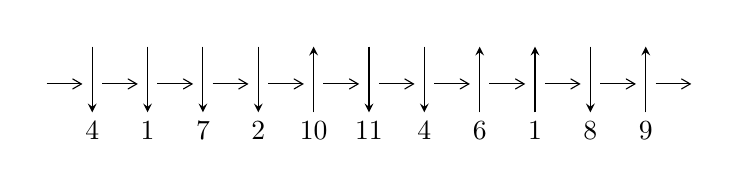
\begin{tikzpicture}[x=20pt, y=17pt]
	% nodes
	\node (C0) at (0, 0) {};
	\node (C1) at (1, 0) {};
	\node (C1U) at (1, +1) {};
	\node (C1D) at (1, -1) {4};

	\node (C2) at (2, 0) {};
	\node (C2U) at (2, +1) {};
	\node (C2D) at (2, -1) {1};

	\node (C3) at (3, 0) {};
	\node (C3U) at (3, +1) {};
	\node (C3D) at (3, -1) {7};

	\node (C4) at (4, 0) {};
	\node (C4U) at (4, +1) {};
	\node (C4D) at (4, -1) {2};

	\node (C5) at (5, 0) {};
	\node (C5U) at (5, +1) {};
	\node (C5D) at (5, -1) {10};

	\node (C6) at (6, 0) {};
	\node (C6U) at (6, +1) {};
	\node (C6D) at (6, -1) {11};

	\node (C7) at (7, 0) {};
	\node (C7U) at (7, +1) {};
	\node (C7D) at (7, -1) {4};

	\node (C8) at (8, 0) {};
	\node (C8U) at (8, +1) {};
	\node (C8D) at (8, -1) {6};

	\node (C9) at (9, 0) {};
	\node (C9U) at (9, +1) {};
	\node (C9D) at (9, -1) {1};

	\node (C10) at (10, 0) {};
	\node (C10U) at (10, +1) {};
	\node (C10D) at (10, -1) {8};

	\node (C11) at (11, 0) {};
	\node (C11U) at (11, +1) {};
	\node (C11D) at (11, -1) {9};
	\node (C12) at (12, 0) {};

	% arrows
	\draw[->,>={angle 60}]
	(C0) edge (C1) (C1) edge (C2) (C2) edge (C3) (C3) edge (C4) (C4) edge (C5) (C5) edge (C6) (C6) edge (C7) (C7) edge (C8) (C8) edge (C9) (C9) edge (C10) (C10) edge (C11) (C11) edge (C12) ;	\draw[->,>=stealth]
	(C1U) edge (C1D) (C2U) edge (C2D) (C3U) edge (C3D) (C4U) edge (C4D) (C5D) edge (C5U) (C6U) edge (C6D) (C7U) edge (C7D) (C8D) edge (C8U) (C9D) edge (C9U) (C10U) edge (C10D) (C11D) edge (C11U) ;
	\end{tikzpicture} \\
\hhline{~~} \\& 
\textbf{Solving Sequence} \\ \cline{2-2} 
 &
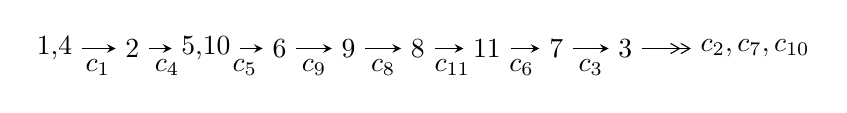
\begin{tikzpicture}[x=25pt, y=7pt]
	% node
	\node (A0) at (-1/8, 0) {1,4};
	\node (A1) at (1, 0) {2};
	\node (A2) at (33/16, 0) {5,10};
	\node (A3) at (25/8, 0) {6};
	\node (A4) at (33/8, 0) {9};
	\node (A5) at (41/8, 0) {8};
	\node (A6) at (49/8, 0) {11};
	\node (A7) at (57/8, 0) {7};
	\node (A8) at (65/8, 0) {3};
	\node (C1) at (1/2, -1) {$c_{1}$};
	\node (C2) at (3/2, -1) {$c_{4}$};
	\node (C3) at (21/8, -1) {$c_{5}$};
	\node (C4) at (29/8, -1) {$c_{9}$};
	\node (C5) at (37/8, -1) {$c_{8}$};
	\node (C6) at (45/8, -1) {$c_{11}$};
	\node (C7) at (53/8, -1) {$c_{6}$};
	\node (C8) at (61/8, -1) {$c_{3}$};
	\node (A9) at (10, 0) {$c_{2},c_{7},c_{10}$};

	% edge
	\draw[->,>=stealth]	
	(A0) edge (A1) (A1) edge (A2) (A2) edge (A3) (A3) edge (A4) (A4) edge (A5) (A5) edge (A6) (A6) edge (A7) (A7) edge (A8) ;
	\draw[->>,>={angle 60}]	
	(A8) edge (A9);
\end{tikzpicture} \\ 

\end{tabular} \\

\footnotetext{
The image of knot diagram is generated by the software ``\textbf{Draw programme}" developed by Andrew Bartholomew(\url{http://www.layer8.co.uk/maths/draw/index.htm\#Running-draw}), where we modified some parts for our purpose(\url{https://github.com/CATsTAILs/LinksPainter}).
}\phantom \\ \newline 
\centering \textbf{Ideals for irreducible components\footnotemark of $X_{\text{par}}$} 
 
\begin{align*}
I^u_{1}&=\langle 
-4.55071\times10^{32} u^{40}-3.04971\times10^{33} u^{39}+\cdots+3.54634\times10^{33} b+1.97956\times10^{32},\\
\phantom{I^u_{1}}&\phantom{= \langle  }-1.27956\times10^{33} u^{40}-7.27594\times10^{33} u^{39}+\cdots+3.54634\times10^{33} a-1.00211\times10^{34},\;u^{41}+7 u^{40}+\cdots+2 u+1\rangle \\
I^u_{2}&=\langle 
b- a+1,\;a^5-4 a^4+4 a^3+a^2-2 a-1,\;u-1\rangle \\
I^u_{3}&=\langle 
b-1,\;-2 u^2+a-4 u-3,\;u^3+u^2-1\rangle \\
\\
\end{align*}
\raggedright * 3 irreducible components of $\dim_{\mathbb{C}}=0$, with total 49 representations.\\
\footnotetext{All coefficients of polynomials are rational numbers. But the coefficients are sometimes approximated in decimal forms when there is not enough margin.}
\newpage
\renewcommand{\arraystretch}{1}
\centering \section*{I. $I^u_{1}= \langle -4.55\times10^{32} u^{40}-3.05\times10^{33} u^{39}+\cdots+3.55\times10^{33} b+1.98\times10^{32},\;-1.28\times10^{33} u^{40}-7.28\times10^{33} u^{39}+\cdots+3.55\times10^{33} a-1.00\times10^{34},\;u^{41}+7 u^{40}+\cdots+2 u+1 \rangle$}
\flushleft \textbf{(i) Arc colorings}\\
\begin{tabular}{m{7pt} m{180pt} m{7pt} m{180pt} }
\flushright $a_{1}=$&$\begin{pmatrix}1\\0\end{pmatrix}$ \\
\flushright $a_{4}=$&$\begin{pmatrix}0\\u\end{pmatrix}$ \\
\flushright $a_{2}=$&$\begin{pmatrix}1\\u^2\end{pmatrix}$ \\
\flushright $a_{5}=$&$\begin{pmatrix}- u\\- u^3+u\end{pmatrix}$ \\
\flushright $a_{10}=$&$\begin{pmatrix}0.360812 u^{40}+2.05167 u^{39}+\cdots-8.17453 u+2.82576\\0.128321 u^{40}+0.859959 u^{39}+\cdots-3.73417 u-0.0558198\end{pmatrix}$ \\
\flushright $a_{6}=$&$\begin{pmatrix}2.57419 u^{40}+13.6219 u^{39}+\cdots-13.2764 u+5.50487\\-0.824828 u^{40}-4.46073 u^{39}+\cdots-3.42158 u-0.703781\end{pmatrix}$ \\
\flushright $a_{9}=$&$\begin{pmatrix}0.232491 u^{40}+1.19171 u^{39}+\cdots-4.44036 u+2.88158\\0.128321 u^{40}+0.859959 u^{39}+\cdots-3.73417 u-0.0558198\end{pmatrix}$ \\
\flushright $a_{8}=$&$\begin{pmatrix}1.89468 u^{40}+10.8589 u^{39}+\cdots-3.67648 u+4.04534\\-0.427689 u^{40}-2.12225 u^{39}+\cdots-3.33185 u+0.204351\end{pmatrix}$ \\
\flushright $a_{11}=$&$\begin{pmatrix}-0.101116 u^{40}-0.258346 u^{39}+\cdots+7.23983 u-3.55682\\0.153838 u^{40}+0.879491 u^{39}+\cdots+4.81960 u+0.645350\end{pmatrix}$ \\
\flushright $a_{7}=$&$\begin{pmatrix}1.89468 u^{40}+10.8589 u^{39}+\cdots-3.67648 u+4.04534\\-4.09416 u^{40}-22.1611 u^{39}+\cdots-6.24482 u-2.19947\end{pmatrix}$ \\
\flushright $a_{3}=$&$\begin{pmatrix}- u^2+1\\u^2\end{pmatrix}$\\ \flushright $a_{3}=$&$\begin{pmatrix}- u^2+1\\u^2\end{pmatrix}$\\&\end{tabular}
\flushleft \textbf{(ii) Obstruction class $= -1$}\\~\\
\flushleft \textbf{(iii) Cusp Shapes $= 9.46225 u^{40}+53.2125 u^{39}+\cdots+10.2497 u+12.8539$}\\~\\
\newpage\renewcommand{\arraystretch}{1}
\flushleft \textbf{(iv) u-Polynomials at the component}\newline \\
\begin{tabular}{m{50pt}|m{274pt}}
Crossings & \hspace{64pt}u-Polynomials at each crossing \\
\hline $$\begin{aligned}c_{1},c_{4}\end{aligned}$$&$\begin{aligned}
&u^{41}-7 u^{40}+\cdots+2 u-1
\end{aligned}$\\
\hline $$\begin{aligned}c_{2}\end{aligned}$$&$\begin{aligned}
&u^{41}+43 u^{40}+\cdots+12 u+1
\end{aligned}$\\
\hline $$\begin{aligned}c_{3},c_{7}\end{aligned}$$&$\begin{aligned}
&u^{41}+2 u^{40}+\cdots+96 u+32
\end{aligned}$\\
\hline $$\begin{aligned}c_{5}\end{aligned}$$&$\begin{aligned}
&u^{41}+16 u^{39}+\cdots-1085 u-79
\end{aligned}$\\
\hline $$\begin{aligned}c_{6}\end{aligned}$$&$\begin{aligned}
&u^{41}+4 u^{40}+\cdots-237 u+191
\end{aligned}$\\
\hline $$\begin{aligned}c_{8}\end{aligned}$$&$\begin{aligned}
&u^{41}+3 u^{40}+\cdots-2 u-1
\end{aligned}$\\
\hline $$\begin{aligned}c_{9},c_{11}\end{aligned}$$&$\begin{aligned}
&u^{41}+5 u^{40}+\cdots+119 u+1
\end{aligned}$\\
\hline $$\begin{aligned}c_{10}\end{aligned}$$&$\begin{aligned}
&u^{41}-6 u^{40}+\cdots+156 u-8
\end{aligned}$\\
\hline
\end{tabular}\\~\\
\newpage\renewcommand{\arraystretch}{1}
\flushleft \textbf{(v) Riley Polynomials at the component}\newline \\
\begin{tabular}{m{50pt}|m{274pt}}
Crossings & \hspace{64pt}Riley Polynomials at each crossing \\
\hline $$\begin{aligned}c_{1},c_{4}\end{aligned}$$&$\begin{aligned}
&y^{41}-43 y^{40}+\cdots+12 y-1
\end{aligned}$\\
\hline $$\begin{aligned}c_{2}\end{aligned}$$&$\begin{aligned}
&y^{41}-83 y^{40}+\cdots+1144 y-1
\end{aligned}$\\
\hline $$\begin{aligned}c_{3},c_{7}\end{aligned}$$&$\begin{aligned}
&y^{41}-30 y^{40}+\cdots+3584 y-1024
\end{aligned}$\\
\hline $$\begin{aligned}c_{5}\end{aligned}$$&$\begin{aligned}
&y^{41}+32 y^{40}+\cdots+183721 y-6241
\end{aligned}$\\
\hline $$\begin{aligned}c_{6}\end{aligned}$$&$\begin{aligned}
&y^{41}+8 y^{40}+\cdots+999709 y-36481
\end{aligned}$\\
\hline $$\begin{aligned}c_{8}\end{aligned}$$&$\begin{aligned}
&y^{41}-11 y^{40}+\cdots+26 y-1
\end{aligned}$\\
\hline $$\begin{aligned}c_{9},c_{11}\end{aligned}$$&$\begin{aligned}
&y^{41}-21 y^{40}+\cdots+13495 y-1
\end{aligned}$\\
\hline $$\begin{aligned}c_{10}\end{aligned}$$&$\begin{aligned}
&y^{41}-18 y^{40}+\cdots+7824 y-64
\end{aligned}$\\
\hline
\end{tabular}\\~\\
\newpage\flushleft \textbf{(vi) Complex Volumes and Cusp Shapes}
$$\begin{array}{c|c|c}  
\text{Solutions to }I^u_{1}& \I (\text{vol} + \sqrt{-1}CS) & \text{Cusp shape}\\
 \hline 
\begin{aligned}
u &= \phantom{-}0.387590 + 0.911908 I \\
a &= -0.971331 - 0.325235 I \\
b &= \phantom{-}0.764541 - 0.597354 I\end{aligned}
 & -2.61027 - 2.03740 I & -5.72892 + 3.65159 I \\ \hline\begin{aligned}
u &= \phantom{-}0.387590 - 0.911908 I \\
a &= -0.971331 + 0.325235 I \\
b &= \phantom{-}0.764541 + 0.597354 I\end{aligned}
 & -2.61027 + 2.03740 I & -5.72892 - 3.65159 I \\ \hline\begin{aligned}
u &= \phantom{-}0.695393 + 0.752192 I \\
a &= -0.0733729 + 0.1016160 I \\
b &= \phantom{-}0.382217 + 0.951284 I\end{aligned}
 & -3.58550 - 3.36599 I & -6.85826 + 4.39505 I \\ \hline\begin{aligned}
u &= \phantom{-}0.695393 - 0.752192 I \\
a &= -0.0733729 - 0.1016160 I \\
b &= \phantom{-}0.382217 - 0.951284 I\end{aligned}
 & -3.58550 + 3.36599 I & -6.85826 - 4.39505 I \\ \hline\begin{aligned}
u &= \phantom{-}0.883212\phantom{ +0.000000I} \\
a &= -5.41324\phantom{ +0.000000I} \\
b &= -1.04711\phantom{ +0.000000I}\end{aligned}
 & \phantom{-}0.458131\phantom{ +0.000000I} & -57.1150\phantom{ +0.000000I} \\ \hline\begin{aligned}
u &= \phantom{-}1.149310 + 0.071261 I \\
a &= -2.67006 + 0.97064 I \\
b &= -0.783716 + 0.351647 I\end{aligned}
 & -0.578838 - 1.255810 I & \phantom{-}2.38019 + 0. I\phantom{ +0.000000I} \\ \hline\begin{aligned}
u &= \phantom{-}1.149310 - 0.071261 I \\
a &= -2.67006 - 0.97064 I \\
b &= -0.783716 - 0.351647 I\end{aligned}
 & -0.578838 + 1.255810 I & \phantom{-}2.38019 + 0. I\phantom{ +0.000000I} \\ \hline\begin{aligned}
u &= \phantom{-}0.508644 + 1.042800 I \\
a &= -0.681098 - 0.649137 I \\
b &= \phantom{-}1.178240 - 0.659530 I\end{aligned}
 & -1.17487 - 9.23550 I & \phantom{-0.000000 -}0. + 7.03311 I \\ \hline\begin{aligned}
u &= \phantom{-}0.508644 - 1.042800 I \\
a &= -0.681098 + 0.649137 I \\
b &= \phantom{-}1.178240 + 0.659530 I\end{aligned}
 & -1.17487 + 9.23550 I & \phantom{-0.000000 } 0. - 7.03311 I \\ \hline\begin{aligned}
u &= -0.817513 + 0.853964 I \\
a &= -0.255534 + 0.434819 I \\
b &= \phantom{-}0.895543 + 0.128230 I\end{aligned}
 & \phantom{-}4.46595 + 3.11596 I & -9.1421 - 11.7493 I\\
 \hline 
 \end{array}$$\newpage$$\begin{array}{c|c|c}  
\text{Solutions to }I^u_{1}& \I (\text{vol} + \sqrt{-1}CS) & \text{Cusp shape}\\
 \hline 
\begin{aligned}
u &= -0.817513 - 0.853964 I \\
a &= -0.255534 - 0.434819 I \\
b &= \phantom{-}0.895543 - 0.128230 I\end{aligned}
 & \phantom{-}4.46595 - 3.11596 I & -9.1421 + 11.7493 I \\ \hline\begin{aligned}
u &= -0.762796 + 0.059538 I \\
a &= \phantom{-}0.685914 + 0.388453 I \\
b &= \phantom{-}1.354300 + 0.223700 I\end{aligned}
 & \phantom{-}4.65237 + 4.48889 I & \phantom{-}10.07507 - 5.98728 I \\ \hline\begin{aligned}
u &= -0.762796 - 0.059538 I \\
a &= \phantom{-}0.685914 - 0.388453 I \\
b &= \phantom{-}1.354300 - 0.223700 I\end{aligned}
 & \phantom{-}4.65237 - 4.48889 I & \phantom{-}10.07507 + 5.98728 I \\ \hline\begin{aligned}
u &= \phantom{-}0.858145 + 0.924978 I \\
a &= -0.0136488 - 0.1120600 I \\
b &= \phantom{-}0.908643 + 0.588751 I\end{aligned}
 & -2.16828 + 2.66511 I & \phantom{-0.000000 } 0 \\ \hline\begin{aligned}
u &= \phantom{-}0.858145 - 0.924978 I \\
a &= -0.0136488 + 0.1120600 I \\
b &= \phantom{-}0.908643 - 0.588751 I\end{aligned}
 & -2.16828 - 2.66511 I & \phantom{-0.000000 } 0 \\ \hline\begin{aligned}
u &= \phantom{-}0.737003\phantom{ +0.000000I} \\
a &= -0.918962\phantom{ +0.000000I} \\
b &= \phantom{-}0.00861004\phantom{ +0.000000I}\end{aligned}
 & -1.10369\phantom{ +0.000000I} & -8.82470\phantom{ +0.000000I} \\ \hline\begin{aligned}
u &= \phantom{-}0.612280 + 0.220916 I \\
a &= -0.42857 + 4.33330 I \\
b &= -0.908176 - 0.005657 I\end{aligned}
 & \phantom{-}0.484163 - 0.158339 I & \phantom{-}13.38590 + 1.00156 I \\ \hline\begin{aligned}
u &= \phantom{-}0.612280 - 0.220916 I \\
a &= -0.42857 - 4.33330 I \\
b &= -0.908176 + 0.005657 I\end{aligned}
 & \phantom{-}0.484163 + 0.158339 I & \phantom{-}13.38590 - 1.00156 I \\ \hline\begin{aligned}
u &= \phantom{-}0.380775 + 0.454242 I \\
a &= \phantom{-}0.670485 - 0.032746 I \\
b &= -1.007360 + 0.614689 I\end{aligned}
 & \phantom{-}1.43126 - 2.56358 I & \phantom{-}1.01752 + 7.87421 I \\ \hline\begin{aligned}
u &= \phantom{-}0.380775 - 0.454242 I \\
a &= \phantom{-}0.670485 + 0.032746 I \\
b &= -1.007360 - 0.614689 I\end{aligned}
 & \phantom{-}1.43126 + 2.56358 I & \phantom{-}1.01752 - 7.87421 I\\
 \hline 
 \end{array}$$\newpage$$\begin{array}{c|c|c}  
\text{Solutions to }I^u_{1}& \I (\text{vol} + \sqrt{-1}CS) & \text{Cusp shape}\\
 \hline 
\begin{aligned}
u &= \phantom{-}1.46523 + 0.11671 I \\
a &= -0.138455 - 1.392320 I \\
b &= \phantom{-}0.596164 - 0.809978 I\end{aligned}
 & -5.33009 + 0.54259 I & \phantom{-0.000000 } 0 \\ \hline\begin{aligned}
u &= \phantom{-}1.46523 - 0.11671 I \\
a &= -0.138455 + 1.392320 I \\
b &= \phantom{-}0.596164 + 0.809978 I\end{aligned}
 & -5.33009 - 0.54259 I & \phantom{-0.000000 } 0 \\ \hline\begin{aligned}
u &= -1.48400\phantom{ +0.000000I} \\
a &= -0.697477\phantom{ +0.000000I} \\
b &= -1.91952\phantom{ +0.000000I}\end{aligned}
 & -2.98279\phantom{ +0.000000I} & \phantom{-0.000000 } 0 \\ \hline\begin{aligned}
u &= -1.51445 + 0.11394 I \\
a &= -0.47763 - 1.44493 I \\
b &= -1.22246 - 1.14875 I\end{aligned}
 & -4.95010 + 4.48342 I & \phantom{-0.000000 } 0 \\ \hline\begin{aligned}
u &= -1.51445 - 0.11394 I \\
a &= -0.47763 + 1.44493 I \\
b &= -1.22246 + 1.14875 I\end{aligned}
 & -4.95010 - 4.48342 I & \phantom{-0.000000 } 0 \\ \hline\begin{aligned}
u &= -1.56483 + 0.05519 I \\
a &= \phantom{-}0.05994 - 1.52905 I \\
b &= -1.049240 - 0.368090 I\end{aligned}
 & -6.84034 + 1.09870 I & \phantom{-0.000000 } 0 \\ \hline\begin{aligned}
u &= -1.56483 - 0.05519 I \\
a &= \phantom{-}0.05994 + 1.52905 I \\
b &= -1.049240 + 0.368090 I\end{aligned}
 & -6.84034 - 1.09870 I & \phantom{-0.000000 } 0 \\ \hline\begin{aligned}
u &= -1.53570 + 0.38602 I \\
a &= -0.149350 + 1.179900 I \\
b &= \phantom{-}1.157160 + 0.624027 I\end{aligned}
 & -8.77885 + 6.88775 I & \phantom{-0.000000 } 0 \\ \hline\begin{aligned}
u &= -1.53570 - 0.38602 I \\
a &= -0.149350 - 1.179900 I \\
b &= \phantom{-}1.157160 - 0.624027 I\end{aligned}
 & -8.77885 - 6.88775 I & \phantom{-0.000000 } 0 \\ \hline\begin{aligned}
u &= \phantom{-}1.60618 + 0.13682 I \\
a &= \phantom{-}0.489280 - 1.112380 I \\
b &= \phantom{-}1.046200 - 0.671367 I\end{aligned}
 & -3.96071 - 6.10430 I & \phantom{-0.000000 } 0\\
 \hline 
 \end{array}$$\newpage$$\begin{array}{c|c|c}  
\text{Solutions to }I^u_{1}& \I (\text{vol} + \sqrt{-1}CS) & \text{Cusp shape}\\
 \hline 
\begin{aligned}
u &= \phantom{-}1.60618 - 0.13682 I \\
a &= \phantom{-}0.489280 + 1.112380 I \\
b &= \phantom{-}1.046200 + 0.671367 I\end{aligned}
 & -3.96071 + 6.10430 I & \phantom{-0.000000 } 0 \\ \hline\begin{aligned}
u &= -1.61056 + 0.23381 I \\
a &= \phantom{-}0.423955 - 1.249650 I \\
b &= \phantom{-}0.32746 - 1.40800 I\end{aligned}
 & -11.27280 + 7.05517 I & \phantom{-0.000000 } 0 \\ \hline\begin{aligned}
u &= -1.61056 - 0.23381 I \\
a &= \phantom{-}0.423955 + 1.249650 I \\
b &= \phantom{-}0.32746 + 1.40800 I\end{aligned}
 & -11.27280 - 7.05517 I & \phantom{-0.000000 } 0 \\ \hline\begin{aligned}
u &= -1.58766 + 0.38818 I \\
a &= \phantom{-}0.05254 + 1.45672 I \\
b &= \phantom{-}1.36138 + 0.75276 I\end{aligned}
 & -7.9395 + 14.4828 I & \phantom{-0.000000 } 0 \\ \hline\begin{aligned}
u &= -1.58766 - 0.38818 I \\
a &= \phantom{-}0.05254 - 1.45672 I \\
b &= \phantom{-}1.36138 - 0.75276 I\end{aligned}
 & -7.9395 - 14.4828 I & \phantom{-0.000000 } 0 \\ \hline\begin{aligned}
u &= -1.68426 + 0.19522 I \\
a &= \phantom{-}0.197462 - 0.763635 I \\
b &= \phantom{-}0.402639 - 0.808887 I\end{aligned}
 & -11.04370 + 1.47634 I & \phantom{-0.000000 } 0 \\ \hline\begin{aligned}
u &= -1.68426 - 0.19522 I \\
a &= \phantom{-}0.197462 + 0.763635 I \\
b &= \phantom{-}0.402639 + 0.808887 I\end{aligned}
 & -11.04370 - 1.47634 I & \phantom{-0.000000 } 0 \\ \hline\begin{aligned}
u &= -0.213366 + 0.037411 I \\
a &= -1.99525 + 2.11282 I \\
b &= -0.146268 + 0.552391 I\end{aligned}
 & \phantom{-}0.05575 - 1.50352 I & \phantom{-}0.38191 + 4.17550 I \\ \hline\begin{aligned}
u &= -0.213366 - 0.037411 I \\
a &= -1.99525 - 2.11282 I \\
b &= -0.146268 - 0.552391 I\end{aligned}
 & \phantom{-}0.05575 + 1.50352 I & \phantom{-}0.38191 - 4.17550 I \\ \hline\begin{aligned}
u &= \phantom{-}0.059485 + 0.186213 I \\
a &= \phantom{-}2.78956 - 5.11758 I \\
b &= -1.278260 - 0.126441 I\end{aligned}
 & \phantom{-}2.56340 + 0.10081 I & \phantom{-}4.27921 + 2.25595 I\\
 \hline 
 \end{array}$$\newpage$$\begin{array}{c|c|c}  
\text{Solutions to }I^u_{1}& \I (\text{vol} + \sqrt{-1}CS) & \text{Cusp shape}\\
 \hline 
\begin{aligned}
u &= \phantom{-}0.059485 - 0.186213 I \\
a &= \phantom{-}2.78956 + 5.11758 I \\
b &= -1.278260 + 0.126441 I\end{aligned}
 & \phantom{-}2.56340 - 0.10081 I & \phantom{-}4.27921 - 2.25595 I\\
 \hline 
 \end{array}$$\newpage\newpage\renewcommand{\arraystretch}{1}
\centering \section*{II. $I^u_{2}= \langle b- a+1,\;a^5-4 a^4+4 a^3+a^2-2 a-1,\;u-1 \rangle$}
\flushleft \textbf{(i) Arc colorings}\\
\begin{tabular}{m{7pt} m{180pt} m{7pt} m{180pt} }
\flushright $a_{1}=$&$\begin{pmatrix}1\\0\end{pmatrix}$ \\
\flushright $a_{4}=$&$\begin{pmatrix}0\\1\end{pmatrix}$ \\
\flushright $a_{2}=$&$\begin{pmatrix}1\\1\end{pmatrix}$ \\
\flushright $a_{5}=$&$\begin{pmatrix}-1\\0\end{pmatrix}$ \\
\flushright $a_{10}=$&$\begin{pmatrix}a\\a-1\end{pmatrix}$ \\
\flushright $a_{6}=$&$\begin{pmatrix}a^2- a-1\\a^2-2 a+1\end{pmatrix}$ \\
\flushright $a_{9}=$&$\begin{pmatrix}1\\a-1\end{pmatrix}$ \\
\flushright $a_{8}=$&$\begin{pmatrix}0\\a^4-5 a^3+8 a^2-3 a-2\end{pmatrix}$ \\
\flushright $a_{11}=$&$\begin{pmatrix}a\\a^2-2 a+1\end{pmatrix}$ \\
\flushright $a_{7}=$&$\begin{pmatrix}0\\a^4-5 a^3+8 a^2-3 a-2\end{pmatrix}$ \\
\flushright $a_{3}=$&$\begin{pmatrix}0\\1\end{pmatrix}$\\ \flushright $a_{3}=$&$\begin{pmatrix}0\\1\end{pmatrix}$\\&\end{tabular}
\flushleft \textbf{(ii) Obstruction class $= 1$}\\~\\
\flushleft \textbf{(iii) Cusp Shapes $= 3 a^4-5 a^3-5 a^2+7 a-5$}\\~\\
\newpage\renewcommand{\arraystretch}{1}
\flushleft \textbf{(iv) u-Polynomials at the component}\newline \\
\begin{tabular}{m{50pt}|m{274pt}}
Crossings & \hspace{64pt}u-Polynomials at each crossing \\
\hline $$\begin{aligned}c_{1}\end{aligned}$$&$\begin{aligned}
&(u-1)^5
\end{aligned}$\\
\hline $$\begin{aligned}c_{2},c_{4}\end{aligned}$$&$\begin{aligned}
&(u+1)^5
\end{aligned}$\\
\hline $$\begin{aligned}c_{3},c_{7}\end{aligned}$$&$\begin{aligned}
&u^5
\end{aligned}$\\
\hline $$\begin{aligned}c_{5},c_{9}\end{aligned}$$&$\begin{aligned}
&u^5- u^4-2 u^3+u^2+u+1
\end{aligned}$\\
\hline $$\begin{aligned}c_{6}\end{aligned}$$&$\begin{aligned}
&u^5+u^4+2 u^3+u^2+u+1
\end{aligned}$\\
\hline $$\begin{aligned}c_{8}\end{aligned}$$&$\begin{aligned}
&u^5-3 u^4+4 u^3- u^2- u+1
\end{aligned}$\\
\hline $$\begin{aligned}c_{10}\end{aligned}$$&$\begin{aligned}
&u^5- u^4+2 u^3- u^2+u-1
\end{aligned}$\\
\hline $$\begin{aligned}c_{11}\end{aligned}$$&$\begin{aligned}
&u^5+u^4-2 u^3- u^2+u-1
\end{aligned}$\\
\hline
\end{tabular}\\~\\
\newpage\renewcommand{\arraystretch}{1}
\flushleft \textbf{(v) Riley Polynomials at the component}\newline \\
\begin{tabular}{m{50pt}|m{274pt}}
Crossings & \hspace{64pt}Riley Polynomials at each crossing \\
\hline $$\begin{aligned}c_{1},c_{2},c_{4}\end{aligned}$$&$\begin{aligned}
&(y-1)^5
\end{aligned}$\\
\hline $$\begin{aligned}c_{3},c_{7}\end{aligned}$$&$\begin{aligned}
&y^5
\end{aligned}$\\
\hline $$\begin{aligned}c_{5},c_{9},c_{11}\end{aligned}$$&$\begin{aligned}
&y^5-5 y^4+8 y^3-3 y^2- y-1
\end{aligned}$\\
\hline $$\begin{aligned}c_{6},c_{10}\end{aligned}$$&$\begin{aligned}
&y^5+3 y^4+4 y^3+y^2- y-1
\end{aligned}$\\
\hline $$\begin{aligned}c_{8}\end{aligned}$$&$\begin{aligned}
&y^5- y^4+8 y^3-3 y^2+3 y-1
\end{aligned}$\\
\hline
\end{tabular}\\~\\
\newpage\flushleft \textbf{(vi) Complex Volumes and Cusp Shapes}
$$\begin{array}{c|c|c}  
\text{Solutions to }I^u_{2}& \I (\text{vol} + \sqrt{-1}CS) & \text{Cusp shape}\\
 \hline 
\begin{aligned}
u &= \phantom{-}1.00000\phantom{ +0.000000I} \\
a &= \phantom{-}1.30992 + 0.54991 I \\
b &= \phantom{-}0.309916 + 0.549911 I\end{aligned}
 & -1.31583 + 1.53058 I & -8.42731 - 4.45807 I \\ \hline\begin{aligned}
u &= \phantom{-}1.00000\phantom{ +0.000000I} \\
a &= \phantom{-}1.30992 - 0.54991 I \\
b &= \phantom{-}0.309916 - 0.549911 I\end{aligned}
 & -1.31583 - 1.53058 I & -8.42731 + 4.45807 I \\ \hline\begin{aligned}
u &= \phantom{-}1.00000\phantom{ +0.000000I} \\
a &= -0.418784 + 0.219165 I \\
b &= -1.41878 + 0.21917 I\end{aligned}
 & \phantom{-}4.22763 - 4.40083 I & -8.55516 + 1.78781 I \\ \hline\begin{aligned}
u &= \phantom{-}1.00000\phantom{ +0.000000I} \\
a &= -0.418784 - 0.219165 I \\
b &= -1.41878 - 0.21917 I\end{aligned}
 & \phantom{-}4.22763 + 4.40083 I & -8.55516 - 1.78781 I \\ \hline\begin{aligned}
u &= \phantom{-}1.00000\phantom{ +0.000000I} \\
a &= \phantom{-}2.21774\phantom{ +0.000000I} \\
b &= \phantom{-}1.21774\phantom{ +0.000000I}\end{aligned}
 & \phantom{-}0.756147\phantom{ +0.000000I} & \phantom{-}3.96490\phantom{ +0.000000I}\\
 \hline 
 \end{array}$$\newpage\newpage\renewcommand{\arraystretch}{1}
\centering \section*{III. $I^u_{3}= \langle b-1,\;-2 u^2+a-4 u-3,\;u^3+u^2-1 \rangle$}
\flushleft \textbf{(i) Arc colorings}\\
\begin{tabular}{m{7pt} m{180pt} m{7pt} m{180pt} }
\flushright $a_{1}=$&$\begin{pmatrix}1\\0\end{pmatrix}$ \\
\flushright $a_{4}=$&$\begin{pmatrix}0\\u\end{pmatrix}$ \\
\flushright $a_{2}=$&$\begin{pmatrix}1\\u^2\end{pmatrix}$ \\
\flushright $a_{5}=$&$\begin{pmatrix}- u\\u^2+u-1\end{pmatrix}$ \\
\flushright $a_{10}=$&$\begin{pmatrix}2 u^2+4 u+3\\1\end{pmatrix}$ \\
\flushright $a_{6}=$&$\begin{pmatrix}7 u^2+11 u+9\\2 u^2+3 u\end{pmatrix}$ \\
\flushright $a_{9}=$&$\begin{pmatrix}2 u^2+4 u+2\\1\end{pmatrix}$ \\
\flushright $a_{8}=$&$\begin{pmatrix}- u\\2 u^2+u-2\end{pmatrix}$ \\
\flushright $a_{11}=$&$\begin{pmatrix}2 u^2+4 u+3\\1\end{pmatrix}$ \\
\flushright $a_{7}=$&$\begin{pmatrix}- u\\u^2+u-1\end{pmatrix}$ \\
\flushright $a_{3}=$&$\begin{pmatrix}- u^2+1\\u^2\end{pmatrix}$\\ \flushright $a_{3}=$&$\begin{pmatrix}- u^2+1\\u^2\end{pmatrix}$\\&\end{tabular}
\flushleft \textbf{(ii) Obstruction class $= 1$}\\~\\
\flushleft \textbf{(iii) Cusp Shapes $= 21 u^2+45 u+39$}\\~\\
\newpage\renewcommand{\arraystretch}{1}
\flushleft \textbf{(iv) u-Polynomials at the component}\newline \\
\begin{tabular}{m{50pt}|m{274pt}}
Crossings & \hspace{64pt}u-Polynomials at each crossing \\
\hline $$\begin{aligned}c_{1}\end{aligned}$$&$\begin{aligned}
&u^3+u^2-1
\end{aligned}$\\
\hline $$\begin{aligned}c_{2},c_{7}\end{aligned}$$&$\begin{aligned}
&u^3+u^2+2 u+1
\end{aligned}$\\
\hline $$\begin{aligned}c_{3}\end{aligned}$$&$\begin{aligned}
&u^3- u^2+2 u-1
\end{aligned}$\\
\hline $$\begin{aligned}c_{4}\end{aligned}$$&$\begin{aligned}
&u^3- u^2+1
\end{aligned}$\\
\hline $$\begin{aligned}c_{5},c_{6}\end{aligned}$$&$\begin{aligned}
&u^3+2 u^2-3 u+1
\end{aligned}$\\
\hline $$\begin{aligned}c_{8}\end{aligned}$$&$\begin{aligned}
&u^3-3 u^2+2 u+1
\end{aligned}$\\
\hline $$\begin{aligned}c_{9}\end{aligned}$$&$\begin{aligned}
&(u+1)^3
\end{aligned}$\\
\hline $$\begin{aligned}c_{10}\end{aligned}$$&$\begin{aligned}
&u^3
\end{aligned}$\\
\hline $$\begin{aligned}c_{11}\end{aligned}$$&$\begin{aligned}
&(u-1)^3
\end{aligned}$\\
\hline
\end{tabular}\\~\\
\newpage\renewcommand{\arraystretch}{1}
\flushleft \textbf{(v) Riley Polynomials at the component}\newline \\
\begin{tabular}{m{50pt}|m{274pt}}
Crossings & \hspace{64pt}Riley Polynomials at each crossing \\
\hline $$\begin{aligned}c_{1},c_{4}\end{aligned}$$&$\begin{aligned}
&y^3- y^2+2 y-1
\end{aligned}$\\
\hline $$\begin{aligned}c_{2},c_{3},c_{7}\end{aligned}$$&$\begin{aligned}
&y^3+3 y^2+2 y-1
\end{aligned}$\\
\hline $$\begin{aligned}c_{5},c_{6}\end{aligned}$$&$\begin{aligned}
&y^3-10 y^2+5 y-1
\end{aligned}$\\
\hline $$\begin{aligned}c_{8}\end{aligned}$$&$\begin{aligned}
&y^3-5 y^2+10 y-1
\end{aligned}$\\
\hline $$\begin{aligned}c_{9},c_{11}\end{aligned}$$&$\begin{aligned}
&(y-1)^3
\end{aligned}$\\
\hline $$\begin{aligned}c_{10}\end{aligned}$$&$\begin{aligned}
&y^3
\end{aligned}$\\
\hline
\end{tabular}\\~\\
\newpage\flushleft \textbf{(vi) Complex Volumes and Cusp Shapes}
$$\begin{array}{c|c|c}  
\text{Solutions to }I^u_{3}& \I (\text{vol} + \sqrt{-1}CS) & \text{Cusp shape}\\
 \hline 
\begin{aligned}
u &= -0.877439 + 0.744862 I \\
a &= -0.079596 + 0.365165 I \\
b &= \phantom{-}1.00000\phantom{ +0.000000I}\end{aligned}
 & \phantom{-}4.66906 + 2.82812 I & \phantom{-}4.03193 + 6.06881 I \\ \hline\begin{aligned}
u &= -0.877439 - 0.744862 I \\
a &= -0.079596 - 0.365165 I \\
b &= \phantom{-}1.00000\phantom{ +0.000000I}\end{aligned}
 & \phantom{-}4.66906 - 2.82812 I & \phantom{-}4.03193 - 6.06881 I \\ \hline\begin{aligned}
u &= \phantom{-}0.754878\phantom{ +0.000000I} \\
a &= \phantom{-}7.15919\phantom{ +0.000000I} \\
b &= \phantom{-}1.00000\phantom{ +0.000000I}\end{aligned}
 & \phantom{-}0.531480\phantom{ +0.000000I} & \phantom{-}84.9360\phantom{ +0.000000I}\\
 \hline 
 \end{array}$$\newpage
\newpage\renewcommand{\arraystretch}{1}
\centering \section*{ IV. u-Polynomials}
\begin{tabular}{m{50pt}|m{274pt}}
Crossings & \hspace{64pt}u-Polynomials at each crossing \\
\hline $$\begin{aligned}c_{1}\end{aligned}$$&$\begin{aligned}
&((u-1)^5)(u^3+u^2-1)(u^{41}-7 u^{40}+\cdots+2 u-1)
\end{aligned}$\\
\hline $$\begin{aligned}c_{2}\end{aligned}$$&$\begin{aligned}
&((u+1)^5)(u^3+u^2+2 u+1)(u^{41}+43 u^{40}+\cdots+12 u+1)
\end{aligned}$\\
\hline $$\begin{aligned}c_{3}\end{aligned}$$&$\begin{aligned}
&u^5(u^3- u^2+2 u-1)(u^{41}+2 u^{40}+\cdots+96 u+32)
\end{aligned}$\\
\hline $$\begin{aligned}c_{4}\end{aligned}$$&$\begin{aligned}
&((u+1)^5)(u^3- u^2+1)(u^{41}-7 u^{40}+\cdots+2 u-1)
\end{aligned}$\\
\hline $$\begin{aligned}c_{5}\end{aligned}$$&$\begin{aligned}
&(u^3+2 u^2-3 u+1)(u^5- u^4-2 u^3+u^2+u+1)\\
&\cdot(u^{41}+16 u^{39}+\cdots-1085 u-79)
\end{aligned}$\\
\hline $$\begin{aligned}c_{6}\end{aligned}$$&$\begin{aligned}
&(u^3+2 u^2-3 u+1)(u^5+u^4+2 u^3+u^2+u+1)\\
&\cdot(u^{41}+4 u^{40}+\cdots-237 u+191)
\end{aligned}$\\
\hline $$\begin{aligned}c_{7}\end{aligned}$$&$\begin{aligned}
&u^5(u^3+u^2+2 u+1)(u^{41}+2 u^{40}+\cdots+96 u+32)
\end{aligned}$\\
\hline $$\begin{aligned}c_{8}\end{aligned}$$&$\begin{aligned}
&(u^3-3 u^2+2 u+1)(u^5-3 u^4+4 u^3- u^2- u+1)\\
&\cdot(u^{41}+3 u^{40}+\cdots-2 u-1)
\end{aligned}$\\
\hline $$\begin{aligned}c_{9}\end{aligned}$$&$\begin{aligned}
&((u+1)^3)(u^5- u^4+\cdots+u+1)(u^{41}+5 u^{40}+\cdots+119 u+1)
\end{aligned}$\\
\hline $$\begin{aligned}c_{10}\end{aligned}$$&$\begin{aligned}
&u^3(u^5- u^4+\cdots+u-1)(u^{41}-6 u^{40}+\cdots+156 u-8)
\end{aligned}$\\
\hline $$\begin{aligned}c_{11}\end{aligned}$$&$\begin{aligned}
&((u-1)^3)(u^5+u^4+\cdots+u-1)(u^{41}+5 u^{40}+\cdots+119 u+1)
\end{aligned}$\\
\hline
\end{tabular}\newpage\renewcommand{\arraystretch}{1}
\centering \section*{ V. Riley Polynomials}
\begin{tabular}{m{50pt}|m{274pt}}
Crossings & \hspace{64pt}Riley Polynomials at each crossing \\
\hline $$\begin{aligned}c_{1},c_{4}\end{aligned}$$&$\begin{aligned}
&((y-1)^5)(y^3- y^2+2 y-1)(y^{41}-43 y^{40}+\cdots+12 y-1)
\end{aligned}$\\
\hline $$\begin{aligned}c_{2}\end{aligned}$$&$\begin{aligned}
&((y-1)^5)(y^3+3 y^2+2 y-1)(y^{41}-83 y^{40}+\cdots+1144 y-1)
\end{aligned}$\\
\hline $$\begin{aligned}c_{3},c_{7}\end{aligned}$$&$\begin{aligned}
&y^5(y^3+3 y^2+2 y-1)(y^{41}-30 y^{40}+\cdots+3584 y-1024)
\end{aligned}$\\
\hline $$\begin{aligned}c_{5}\end{aligned}$$&$\begin{aligned}
&(y^3-10 y^2+5 y-1)(y^5-5 y^4+8 y^3-3 y^2- y-1)\\
&\cdot(y^{41}+32 y^{40}+\cdots+183721 y-6241)
\end{aligned}$\\
\hline $$\begin{aligned}c_{6}\end{aligned}$$&$\begin{aligned}
&(y^3-10 y^2+5 y-1)(y^5+3 y^4+4 y^3+y^2- y-1)\\
&\cdot(y^{41}+8 y^{40}+\cdots+999709 y-36481)
\end{aligned}$\\
\hline $$\begin{aligned}c_{8}\end{aligned}$$&$\begin{aligned}
&(y^3-5 y^2+10 y-1)(y^5- y^4+8 y^3-3 y^2+3 y-1)\\
&\cdot(y^{41}-11 y^{40}+\cdots+26 y-1)
\end{aligned}$\\
\hline $$\begin{aligned}c_{9},c_{11}\end{aligned}$$&$\begin{aligned}
&((y-1)^3)(y^5-5 y^4+\cdots- y-1)(y^{41}-21 y^{40}+\cdots+13495 y-1)
\end{aligned}$\\
\hline $$\begin{aligned}c_{10}\end{aligned}$$&$\begin{aligned}
&y^3(y^5+3 y^4+\cdots- y-1)(y^{41}-18 y^{40}+\cdots+7824 y-64)
\end{aligned}$\\
\hline
\end{tabular}
\vskip 2pc
\end{document}